\documentclass[12pt, oneside]{article}

\usepackage[letterpaper, scale=0.89, centering]{geometry}
\usepackage{fancyhdr}
\setlength{\parindent}{0em}
\setlength{\parskip}{1em}

\usepackage{tikz}
\usetikzlibrary{automata,positioning,arrows}

\pagestyle{fancy}
\fancyhf{}
\renewcommand{\headrulewidth}{0pt}
\rfoot{\href{https://creativecommons.org/licenses/by-nc-sa/2.0/}{CC BY-NC-SA 2.0} Version \today~(\thepage)}

\usepackage{amssymb,amsmath,pifont,amsfonts,comment,enumerate,enumitem}
\usepackage{currfile,xstring,hyperref,tabularx,graphicx,wasysym}
\usepackage[labelformat=empty]{caption}
\usepackage{xcolor}
\usepackage{multicol,multirow,array,listings,tabularx,lastpage,textcomp,booktabs}

\lstnewenvironment{algorithm}[1][] {   
    \lstset{ mathescape=true,
        frame=tB,
        numbers=left, 
        numberstyle=\tiny,
        basicstyle=\rmfamily\scriptsize, 
        keywordstyle=\color{black}\bfseries,
        keywords={,procedure, div, for, to, input, output, return, datatype, function, in, if, else, foreach, while, begin, end, }
        numbers=left,
        xleftmargin=.04\textwidth,
        #1
    }
}
{}

\newcommand\abs[1]{\lvert~#1~\rvert}
\newcommand{\st}{\mid}

\newcommand{\cmark}{\ding{51}}
\newcommand{\xmark}{\ding{55}}
 
\begin{document}
\begin{flushright}
    \StrBefore{\currfilename}{.}
\end{flushright} \section*{Week5 monday}


  Three different CFGs that each generate the  language $\{abba\}$
  
  \begin{align*}
  & ( \{ S, T, V, W\}, \{a,b\}, \{ S \to aT, T \to bV, V \to bW, W \to a\}, S)\\
  & \\ 
  & \\ 
  & \\ 
  & ( \{ Q \}, \{a,b\}, \{Q \to abba\}, Q) \\
  & \\ 
  & \\ 
  & \\
  & ( \{ X,Y \}, \{a,b\}, \{X \to aYa, Y \to bb\}, X) 
  & \\ 
  & \\ 
  \end{align*} 

  Design a CFG to generate the  language $\{a^n b^n \mid  n  \geq  0\}$
  
  \vspace{100pt}
  
  {\it Sample derivation:} 
  
  \vspace{30pt}
  
  
  Design a CFG to generate the  language $\{a^i b^j \mid j \geq i  \geq 0\}$
  
  \vspace{100pt}
  
  {\it Sample derivation:} 
  
  \vspace{30pt}

\newpage

{\bf Theorem  2.20}: A language is  generated by some context-free  grammar
if  and only if it is recognized by some push-down automaton.

Definition: a language is called {\bf context-free} if it is the language generated by a context-free grammar.
The class of all context-free language over a given alphabet $\Sigma$ is called {\bf CFL}.

Consequences:
\begin{itemize}
    \item Quick proof that every regular language is context free 
    \item To prove closure of the class of context-free languages under a given operation, we can choose 
    either of two modes 
    of proof (via CFGs or PDAs) depending on which is easier
    \item To fully specify a PDA we could give its $6$-tuple formal definition or we could give its input 
alphabet, stack alphabet, and state diagram.
An informal description of a PDA is a step-by-step description of how its computations 
would process input strings; the reader should be able to reconstruct the state diagram or formal 
definition precisely from such a descripton. The informal description of a PDA can refer to some 
common modules or subroutines that are computable by PDAs:
\begin{itemize}
  \item PDAs can ``test for emptiness of stack'' without providing details. 
  {\it How?} We can always push a special end-of-stack symbol, $\$$, at the start, before processing
  any input, and then use this symbol as a flag.
  \item PDAs can ``test for end of input'' without providing details.
  {\it How?} We can transform a PDA to one where accepting states are only those reachable 
  when there are no more input symbols.
\end{itemize}

\end{itemize}


Over $\Sigma = \{a,b\}$, let $L = \{ a^n b^m \mid n  \neq m \}$. {\bf Goal}: Prove $L$ is context-free.


\vfill

\newpage
Suppose $L_1$ and $L_2$ are context-free languages over $\Sigma$.  {\bf Goal}:  $L_1 \cup L_2$  is  also context-free.

{\it Approach 1: with  PDAs}

Let $M_1 = ( Q_1, \Sigma, \Gamma_1, \delta_1, q_1, F_1)$ and
$M_2 = ( Q_2, \Sigma, \Gamma_2, \delta_2, q_2, F_2)$ be PDAs with 
$L(M_1) =  L_1$  and  $L(M_2) = L_2$.

Define $M = $

\vfill

{\it Approach  2: with CFGs}

Let $G_1 = (V_1, \Sigma, R_1, S_1)$  and   $G_2 = (V_2, \Sigma, R_2, S_2)$  be CFGs  with
$L(G_1) =  L_1$  and  $L(G_2) = L_2$.

Define $G = $

\vfill

\newpage
Suppose $L_1$ and $L_2$ are context-free languages over $\Sigma$.  {\bf Goal}:  $L_1 \circ L_2$  is  also context-free.


{\it Approach 1: with  PDAs}

Let $M_1 = ( Q_1, \Sigma, \Gamma_1, \delta_1, q_1, F_1)$ and
$M_2 = ( Q_2, \Sigma, \Gamma_2, \delta_2, q_2, F_2)$ be PDAs with 
$L(M_1) =  L_1$  and  $L(M_2) = L_2$.

Define $M = $

\vfill

{\it Approach  2: with CFGs}

Let $G_1 = (V_1, \Sigma, R_1, S_1)$  and   $G_2 = (V_2, \Sigma, R_2, S_2)$  be CFGs  with
$L(G_1) =  L_1$  and  $L(G_2) = L_2$.

Define $G = $

\vfill
\newpage
{\it Summary}

Over a fixed alphabet $\Sigma$, a language $L$ is {\bf regular}

\vspace{-20pt}
\begin{center}
    iff it is described by some regular expression \\
    iff it is recognized by some DFA\\
    iff it is recognized by some NFA
\end{center}

Over a fixed alphabet $\Sigma$, a language $L$ is {\bf context-free}

\vspace{-20pt}
\begin{center}
    iff it is generated by some CFG\\
    iff it is recognized by some PDA
\end{center}

{\bf Fact}: Every regular language is a context-free language.

{\bf Fact}: There are context-free languages that are not nonregular.

{\bf Fact}: There are countably many regular languages.

{\bf Fact}: There are countably inifnitely many context-free languages.

{\it Consequence}: Most languages are {\bf not} context-free!

{\bf Examples  of non-context-free languages}

\begin{align*}
    &\{ a^n b^n c^n \mid 0 \leq n , n \in \mathbb{Z}\}\\
    &\{ a^i b^j c^k \mid 0 \leq i \leq j \leq k , i \in \mathbb{Z}, j \in \mathbb{Z}, k \in \mathbb{Z}\}\\
    &\{ ww \mid w \in \{0,1\}^* \}
\end{align*}
(Sipser Ex 2.36, Ex 2.37, 2.38)

There is a Pumping Lemma for CFL that can be used to prove a specific language is non-context-free: 
If $A$ is a context-free language, there there
is a number $p$ where, if $s$ is any string in $A$ of length at least $p$, then $s$ may be divided 
into five pieces $s = uvxyz$ where (1) for each $i \geq 0$, $uv^ixy^iz \in A$, (2) $|uv|>0$, (3) $|vxy| \leq p$.
{\it We will not go into the details of the proof or application of Pumping Lemma for CFLs this quarter.}
 \vfill
\section*{Week5 wednesday}


    
A set $X$ is said to be {\bf closed} under an operation $OP$ if, for any elements in $X$, applying 
$OP$ to them gives an element in $X$.  


\begin{center}
\begin{tabular}{|c|l|}
\hline
True/False & Closure claim \\
\hline
True &  The set of integers is closed under multiplication. \\
& $\forall x \forall y \left( ~(x \in \mathbb{Z} \wedge y \in \mathbb{Z})\to xy \in \mathbb{Z}~\right)$ \\
\hline
True & For each set $A$, the power set of $A$ is closed under intersection. \\
& $\forall A_1 \forall A_2 \left( ~(A_1 \in \mathcal{P}(A) \wedge A_2 \in \mathcal{P}(A) \in \mathbb{Z}) \to A_1 \cap A_2 \in \mathcal{P}(A)~\right)$ \\
\hline
  & The class of regular languages over $\Sigma$ is closed under complementation. \\
  & \\
 \hline
  & The class of regular languages over $\Sigma$ is closed under union. \\
  & \\
 \hline
  & The class of regular languages over $\Sigma$ is closed under intersection. \\
  & \\
  \hline
  & The class of regular languages over $\Sigma$ is closed under concatenation. \\
  & \\
 \hline
  & The class of regular languages over $\Sigma$ is closed under Kleene star. \\
  & \\
\hline
    & The class of context-free languages over $\Sigma$ is closed under complementation. \\
  & \\
\hline
    & The class of context-free languages over $\Sigma$ is closed under union. \\
  & \\
\hline
    & The class of context-free languages over $\Sigma$ is closed under intersection. \\
  & \\
\hline
    & The class of context-free languages over $\Sigma$ is closed under concatenation. \\
  & \\
\hline
    & The class of context-free languages over $\Sigma$ is closed under Kleene star. \\
  & \\
\hline
\end{tabular}
\end{center}

\vfill

Assume  $\Sigma  = \{0,1, \#\}$
\begin{center}
\begin{tabular}{|cc|}
\hline
&\\
$\Sigma^*$  & Regular ~~/~~ nonregular and context-free ~~/~~not context-free\\

$\{0^i\# 1^j \mid i \geq  0, j  \geq 0\}$  & Regular ~~/~~ nonregular and context-free ~~/~~not context-free\\

$\{0^i1^j\# 1^j0^i \mid i \geq  0, j  \geq 0\}$  & Regular ~~/~~ nonregular and context-free ~~/~~not context-free\\

$\{0^i1^j\# 0^i 1^j \mid i \geq  0, j  \geq 0\}$  & Regular ~~/~~ nonregular and context-free ~~/~~not context-free\\
&\\
\hline
\end{tabular}
\end{center}

\newpage
{\bf Turing machines}: unlimited read + write memory, unlimited time (computation can proceed
without ``consuming'' input and can re-read symbols of input)
\begin{itemize}
\item Division betweeen program (CPU, state diagram) and data
\item Unbounded memory gives theoretical limit to what modern computation 
(including PCs, supercomputers, quantum computers) can achieve
\item State diagram formulation is simple enough to reason about (and diagonalize against) while
expressive enough to capture modern computation
\end{itemize}

For Turing machine $M= (Q, \Sigma, \Gamma, \delta, q_0, q_{accept}, q_{reject})$ 
the {\bf computation} of $M$ on a string $w$ over $\Sigma$  is:

\vspace{-20pt}

\begin{itemize}
\setlength{\itemsep}{0pt}
\item Read/write head starts at leftmost position on tape. 
\item Input string is written on $|w|$-many leftmost cells of tape, 
rest of  the tape cells have  the blank symbol. {\bf Tape alphabet} 
is $\Gamma$ with $\textvisiblespace\in \Gamma$ and $\Sigma \subseteq \Gamma$.
The blank symbol $\textvisiblespace \notin \Sigma$.
\item Given current state of machine and current symbol being read at the tape head, 
the machine transitions to next state, writes a symbol to the current position  of the 
tape  head (overwriting existing symbol), and moves the tape head L or R (if possible). 
Formally, {\bf transition function}  is 
\[
  \delta: Q\times \Gamma \to Q \times \Gamma \times \{L, R\}
\]
\item Computation ends if and when machine enters either the accept or the reject state.
This is called {\bf halting}.
Note: $q_{accept} \neq q_{reject}$.
\end{itemize}

The {\bf language recognized by the  Turing machine} $M$,  is  
\[
  \{ w \in \Sigma^* \mid \textrm{computation of $M$ on $w$ halts after entering the accept state}\} = \{ w \in \Sigma^* \mid w \textrm{ is accepted by } M\}
\]

\newpage
An example Turing machine: $\Sigma = \phantom{\hspace{1in}}, \Gamma = \phantom{\hspace{1in}} $
\[
  \delta ( ( q0, 0)  ) =  
\]

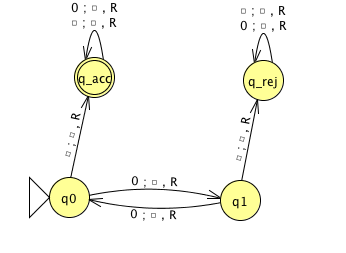
\includegraphics[width=2.5in]{Lect13TM1.png}

Formal definition: 


Sample computation: 

\begin{tabular}{|c|c|c|c|c|c|c|}
\hline
\multicolumn{1}{|c}{$q0\downarrow$} &  \multicolumn{6}{c|}{\phantom{A}}\\
\hline
$0$ & $0$  & $0$ & $\textvisiblespace $& $\textvisiblespace $& $\textvisiblespace $&  $\textvisiblespace $\\
\hline
\multicolumn{7}{|c|}{\phantom{A}}\\
\hline
\phantom{AA} & \phantom{AA}& \phantom{AA}& \phantom{AA}& \phantom{AA}& \phantom{AA}& \phantom{AA} \\
\hline
\multicolumn{7}{|c|}{\phantom{A}}\\
\hline
\phantom{AA} & \phantom{AA}& \phantom{AA}& \phantom{AA}& \phantom{AA}& \phantom{AA}& \phantom{AA} \\
\hline
\multicolumn{7}{|c|}{\phantom{A}}\\
\hline
\phantom{AA} & \phantom{AA}& \phantom{AA}& \phantom{AA}& \phantom{AA}& \phantom{AA}& \phantom{AA} \\
\hline
\multicolumn{7}{|c|}{\phantom{A}}\\
\hline
\phantom{AA} & \phantom{AA}& \phantom{AA}& \phantom{AA}& \phantom{AA}& \phantom{AA}& \phantom{AA} \\
\hline
\end{tabular}

\vfill

The language recognized by this machine is \ldots

{\it Extra practice:}

 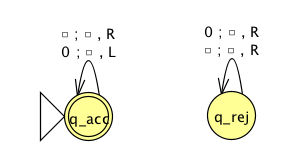
\includegraphics[width=2in]{Lect13TM2.png} 


 Formal definition: 


 Sample computation: 
  \vfill
\end{document}